%! TeX program = lualatex
\documentclass[a4paper]{article} 

\usepackage[backend=biber, style=numeric, date=iso, urldate=iso]{biblatex}
\addbibresource{references.bib}
\DeclareFieldFormat{urldate}{Accessed on: #1}
\usepackage{amsmath}
% packages
\usepackage{microtype}      % Slightly tweak font spacing for aesthetics
\usepackage[english]{babel} % Language hyphenation and typographical rules
\usepackage[final, colorlinks = true, urlcolor = black, linkcolor = black, citecolor = black]{hyperref} 
\usepackage{changepage}     % adjust margins on the fly

\usepackage{fontspec}
\setmainfont{EB Garamond}
\setmonofont[Scale=MatchLowercase]{Deja Vu Sans Mono}

\usepackage{minted}
\usemintedstyle{algol_nu}
\usepackage{xcolor}

\usepackage{pgfplots}
\pgfplotsset{width=\textwidth,compat=1.9}

\usepackage{caption}
\newenvironment{code}{\captionsetup{type=listing}}{}
\captionsetup[listing]{skip=0pt}
\setlength{\abovecaptionskip}{5pt}
\setlength{\belowcaptionskip}{5pt}

\usepackage[yyyymmdd]{datetime}
\renewcommand{\dateseparator}{--}

\usepackage{titlesec}
% \titleformat{\section}{\LARGE\bfseries}{}{}{}[\titlerule]
% \titleformat{\subsection}{\Large\bfseries}{}{0em}{}
% \titlespacing{\subsection}{0em}{-0.7em}{0em}
%
% \titleformat{\subsubsection}{\large\bfseries}{}{0em}{$\bullet$ }
% \titlespacing{\subsubsection}{1em}{-0.7em}{0em}

% margins
\addtolength{\hoffset}{-2.25cm}
\addtolength{\textwidth}{4.5cm}
\addtolength{\voffset}{-3.25cm}
\addtolength{\textheight}{5cm}
\setlength{\parskip}{0pt}
\setlength{\parindent}{0in}
% \setcounter{secnumdepth}{0}

\begin{document}
\hrule \medskip
\begin{minipage}{0.295\textwidth} 
    \raggedright
    \footnotesize 
    \begin{tabular}{@{}l l}
        Name: & Andrew Hayes \\
        Student ID: & 21321503 \\
        E-mail: & \href{mailto://a.hayes18@universityofgalway.ie}{\texttt{a.hayes18@universityofgalway.ie}} \\
    \end{tabular}
\end{minipage}
\begin{minipage}{0.4\textwidth} 
    \centering 
    \vspace{0.4em}
    \LARGE
    \textsc{ct421} \\ 
\end{minipage}
\begin{minipage}{0.295\textwidth} 
    \raggedleft
    \today
\end{minipage}
\medskip\hrule 
\begin{center}
    \normalsize
    Project 2: Evolutionary Game Theory
\end{center}
\hrule
\medskip

\section{Part 1: Evolution Against Fixed Strategies}
\subsection{Implementation}
To implement the genetic algorithm for this assignment, I largely re-used the general framework I developed in the previous assignment, making appropriate changes and removing unnecessary features.
The genetic algorithm can be tuned by providing command-line flags \& arguments, the possible options for which can be displayed by running the program with the \texttt{-h} flag, i.e., 
\mintinline{bash}{python3 ipd.py -h}, which gives the following output:

\begin{code}
\begin{minted}[linenos, breaklines, frame=single]{text}
usage: ipd.py [-h] [-s SIZE] [-g NUM_GENERATIONS] [-a GIVE_UP_AFTER]
              [-i NUM_ITERATIONS] [-p SELECTION_PROPORTION]
              [-c CROSSOVER_RATE] [-m MUTATION_RATE] [-o OUTPUT_FILE]

Program to evolve strategies for the Iterated Prisoner's Dilemma

options:
  -h, --help            show this help message and exit
  -s, --size SIZE       Initial population size
  -g, --num-generations NUM_GENERATIONS
                        Number of generations
  -a, --give-up-after GIVE_UP_AFTER
                        Number of generations to give up after if best
                        solution has remained unchanged
  -i, --num-iterations NUM_ITERATIONS
                        Number of iterations of the dilemma between two agents
  -p, --selection-proportion SELECTION_PROPORTION
                        The proportion of the population to be selected
                        (survive) on each generation
  -c, --crossover-rate CROSSOVER_RATE
                        Probability of a selected pair of solutions to
                        sexually reproduce
  -m, --mutation-rate MUTATION_RATE
                        Probability of a selected offspring to undergo
                        mutation
  -o, --output-file OUTPUT_FILE
                        File to write TSV results to
\end{minted}
\caption{Output of \texttt{python3 ipd.py -h}}
\end{code}

I chose to represent each strategy as a 3-bit string, where \verb|0| represents defection and \verb|1| represents co-operation;
the first bit of the string represents the strategy's first move, the second bit represents the strategy's reaction to a defection by its opponent, and the third bit represents the strategy's reaction to a co-operation by its opponent.
For that reason, there are only eight possible strategies in the search space:
\begin{itemize}
    \item   \verb|[0, 0, 0]|:   always defect.
    \item   \verb|[0, 0, 1]|:   grim tit-for-tat.
    \item   \verb|[0, 1, 0]|:   defect at first, then do opposite of what opponent did last.
    \item   \verb|[0, 1, 1]|:   defect at first, then always co-operate.
    \item   \verb|[1, 0, 0]|:   feint co-operation, then always defect.
    \item   \verb|[1, 0, 1]|:   tit-for-tat.
    \item   \verb|[1, 1, 0]|:   co-operate at first, then do opposite of what opponent did last.
    \item   \verb|[1, 1, 1]|:   always co-operate.
\end{itemize}

Because there are only 8 possibilities in the search space, and the recommended population size in the assignment specification was 50 -- 100, any random initialisation of the population was almost guaranteed to find not only the optimal solution, but every possible solution in the search space (assuming there is one optimal solution out of the eight, and that we randomly initialise 100 individuals, the chances of \textit{not} finding the optimal solution immediately are $\frac{7}{8}^{100} \approx 0.0000015878$).
Therefore, I took the assignment not to focus on finding the optimal solution, but exploring how the population converges on the optimal solution for a given fixed fitness landscape.
This small search space also meant that the population converges very quickly, and quickly sheds diversity in the population;
in an attempt to to mitigate this, I set the mutation rate to be relatively high (0.1), and allowed the number of generations to be longer than necessary so as to observe the population dynamics over time.
My crossover \& mutation operators were also relatively simple to reflect this small search space:
I implemented one crossover operator, that being single-point crossover, and one mutation operator, that being a simple bit-flip mutation.

\subsection{Exploring Convergence with different Fitness Evaluations}
\subsubsection{Equally-Proportioned Always Co-Operate, Always Defect, \& Tit-for-Tat}
When the fitness function consisted of an always co-operate strategy, an always defect strategy, \& a tit-for-tat strategy, the best-performing evolved strategy was \verb|[0,1,0]|: defect on the first move, then do the opposite of what the opponent did last time.
It achieved a fitness of 75, narrowly outperforming its more-polite sibling of \verb|[1,1,0]| (co-operate at first, then do the opposite of what the opponent did) and \verb|[0,0,0]| (always defect), both with fitnesses of 74.
This surprised me at first, but it makes sense:
the strategy of doing the opposite of what the opponent last did performs poorly against Always Defect, as it will lose each time, but exploits Always Co-Operate efficiently, allowing it to gain a high fitness score.
It also does reasonably well against Tit-for-Tat: every second iteration, it will successfully exploit Tit-for-Tat, but lose every other iteration.
The strategy of defecting then doing the opposite of the opponent out-performs its sibling co-operate then do the opposite because it doesn't miss the opportunity to exploit Tit-for-Tat \& Always Co-Operate on its first move.


\begin{figure}[H]
    \centering
    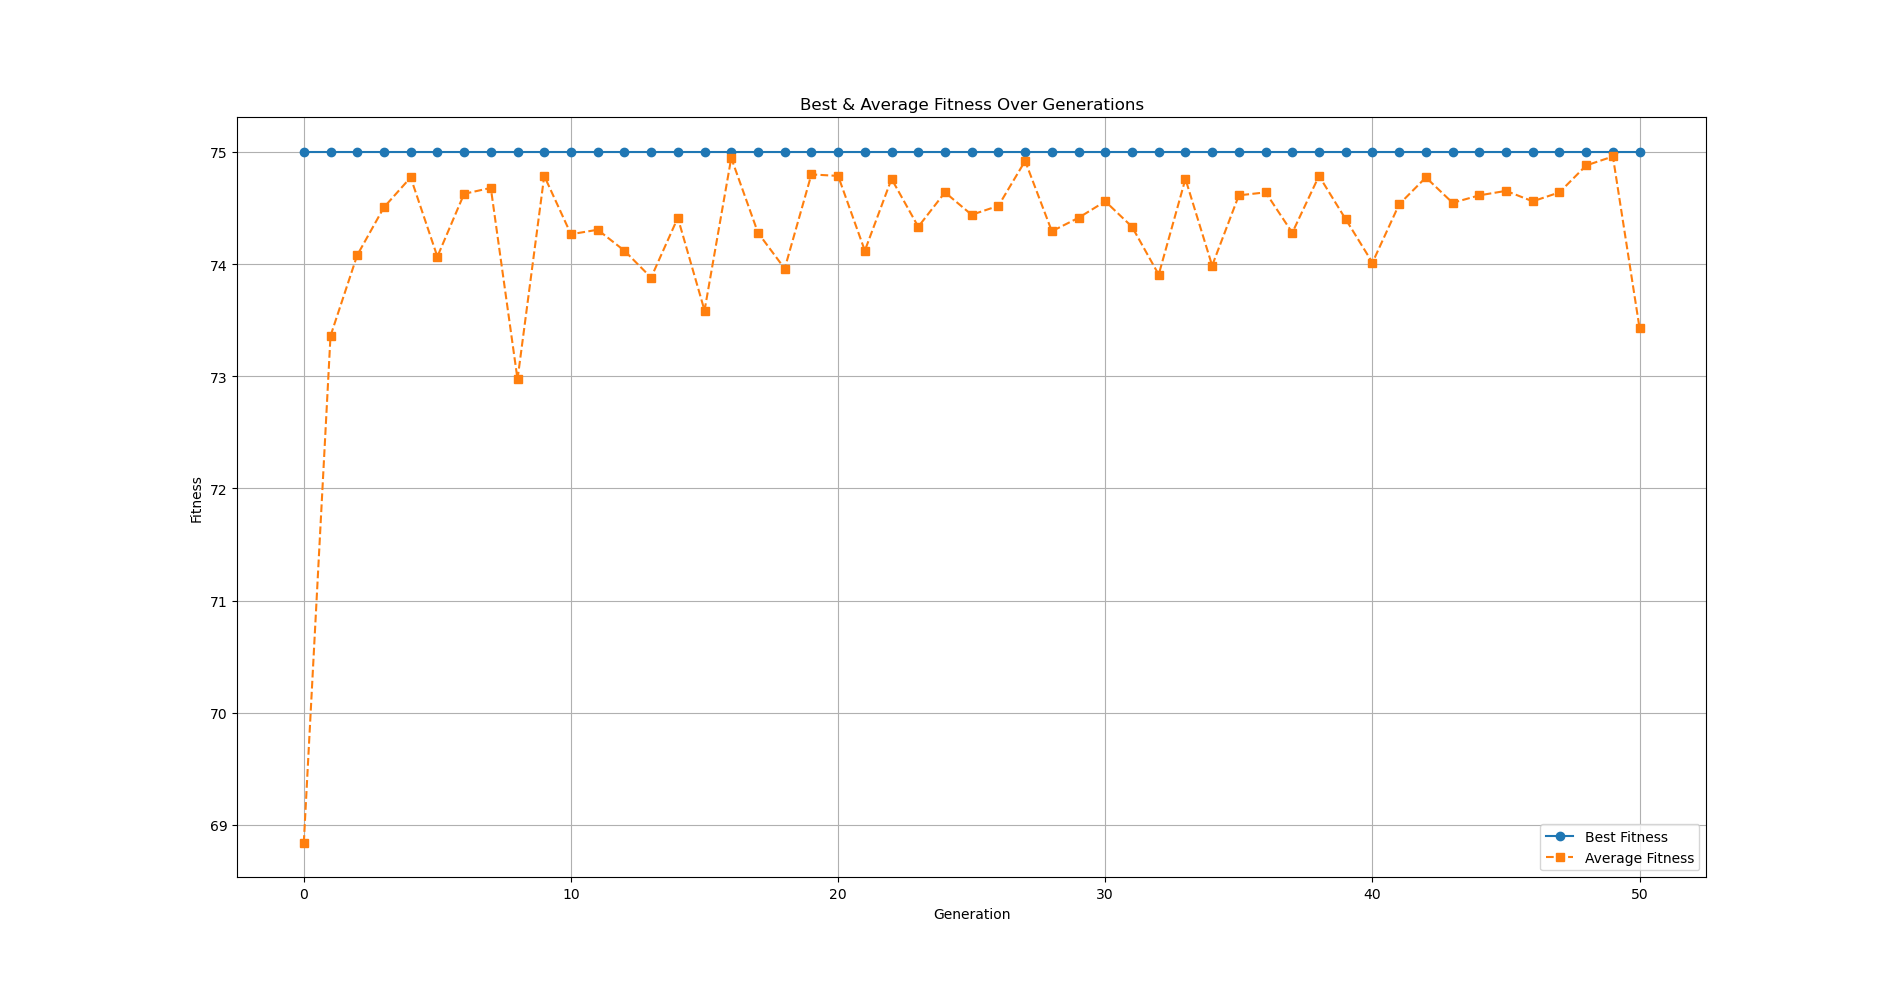
\includegraphics[width=\textwidth]{./images/onefitness.png}
    \caption{ Fitness over generations}
\end{figure}

\begin{figure}[H]
    \centering
    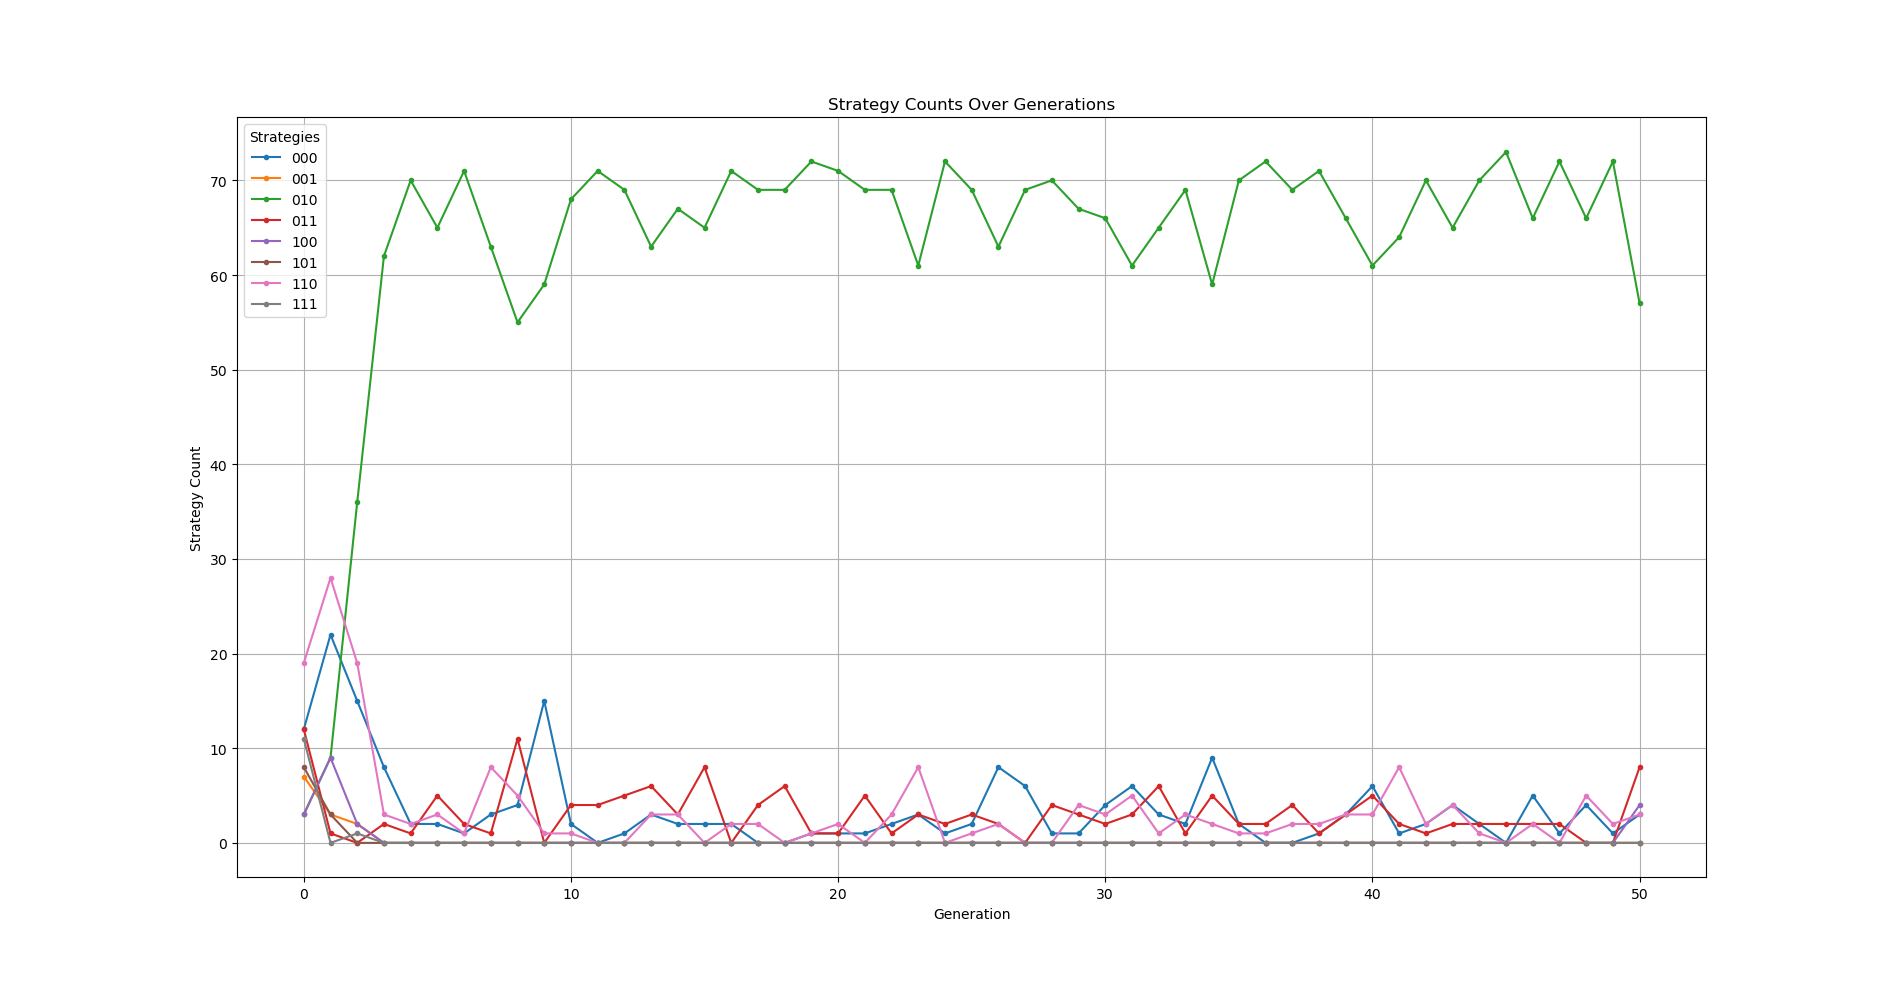
\includegraphics[width=\textwidth]{./images/1strats.png}
    \caption{Diversity of the strategy population over generations}
\end{figure}

\subsubsection{$2 \times $ Always Defect, $1 \times$ Always Co-Operate, \& $1 \times$ Tit-for-Tat}
\begin{code}
\begin{minted}[linenos, breaklines, frame=single]{text}
Best strategy: [0, 0, 0]
Fitness: 84
Generation: 0
[0, 0, 0]: 84
[0, 0, 1]: 77
[0, 1, 0]: 76
[0, 1, 1]: 63
[1, 0, 0]: 82
[1, 0, 1]: 78
[1, 1, 0]: 74
[1, 1, 1]: 60
\end{minted}
\caption{Output of $2 \times $ always defect, $1 \times$ always co-operate, \& $1 \times$ tit-for-tat}
\end{code}

When a second Always Defect is added to the mix, it becomes a better strategy to also always defect:
while this means it will do poorly against Always Defect and Tit-for-Tat, it can efficiently \& ruthlessly exploit the Always Co-Operate to gain a high fitness regardless.

\begin{figure}[H]
    \centering
    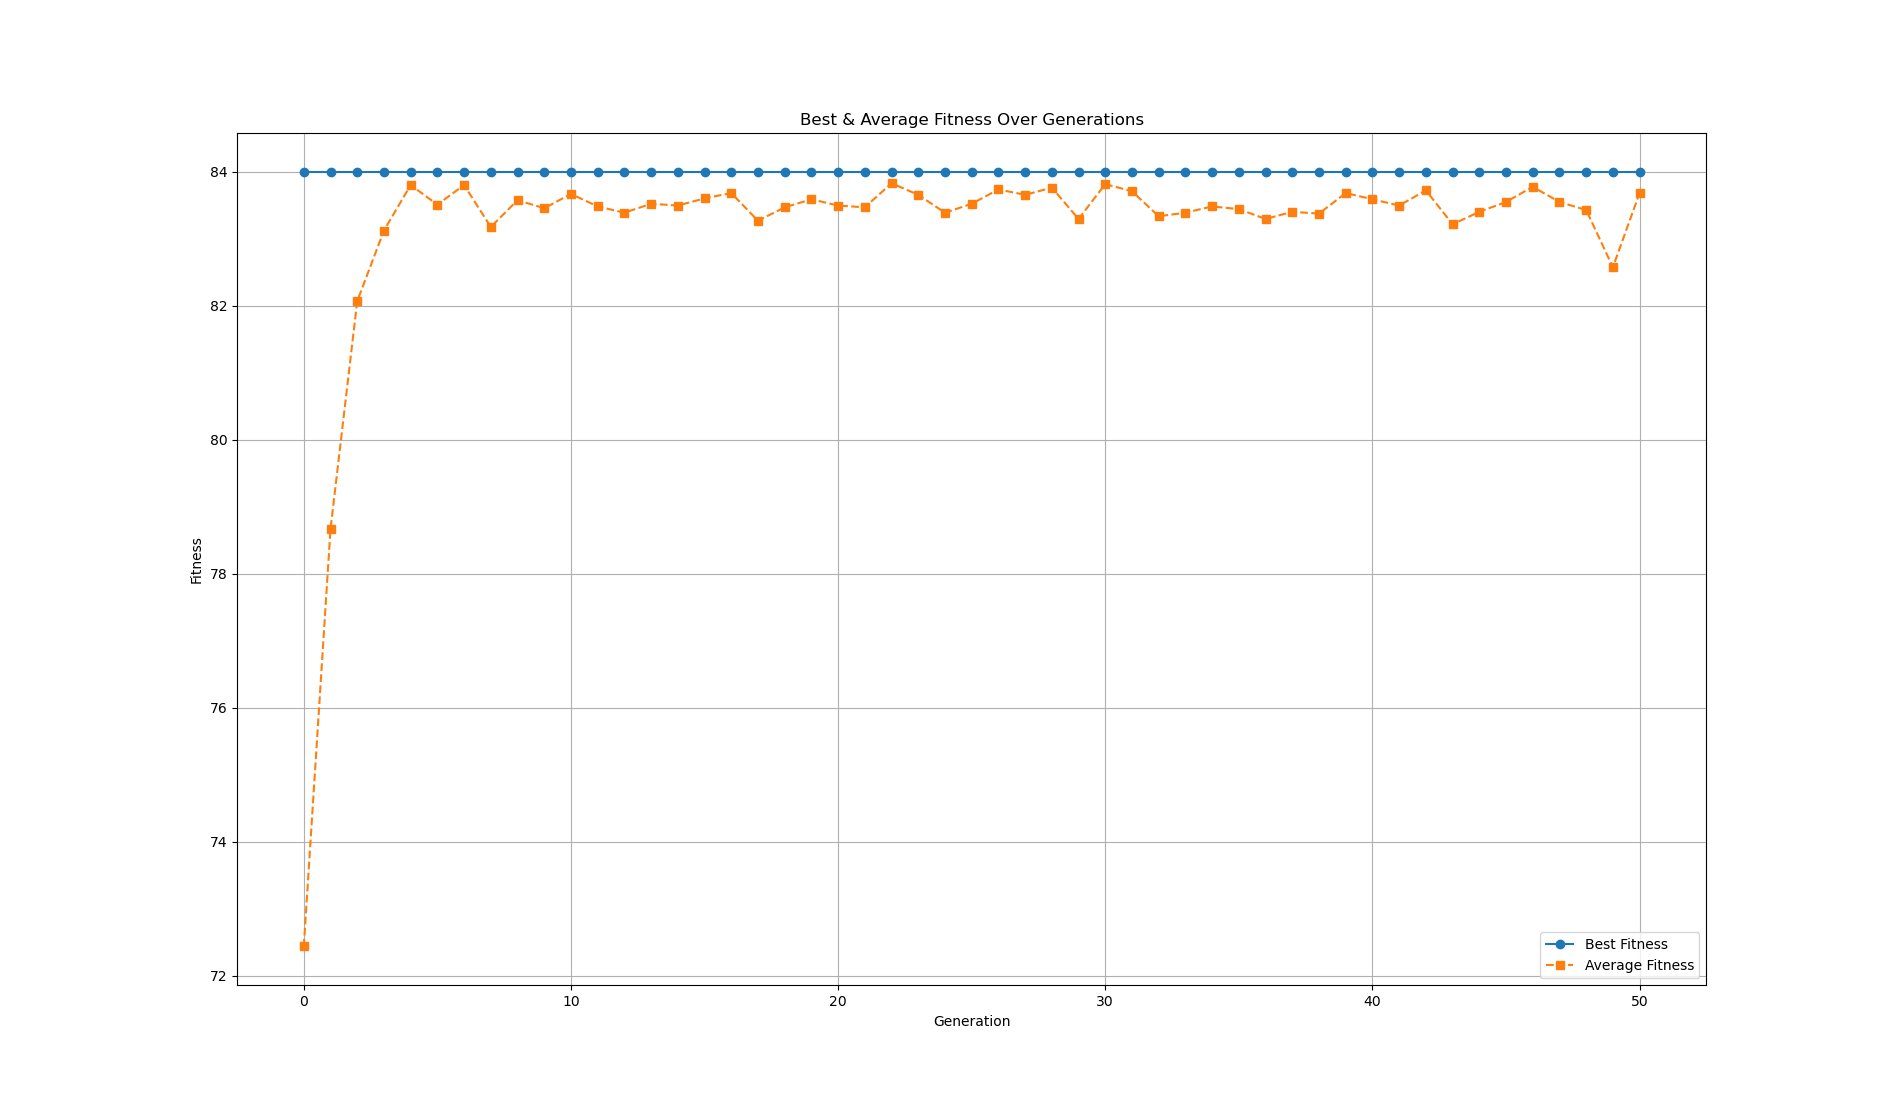
\includegraphics[width=\textwidth]{./images/defect_fitness.png}
    \caption{Fitness over generations}
\end{figure}

\begin{figure}[H]
    \centering
    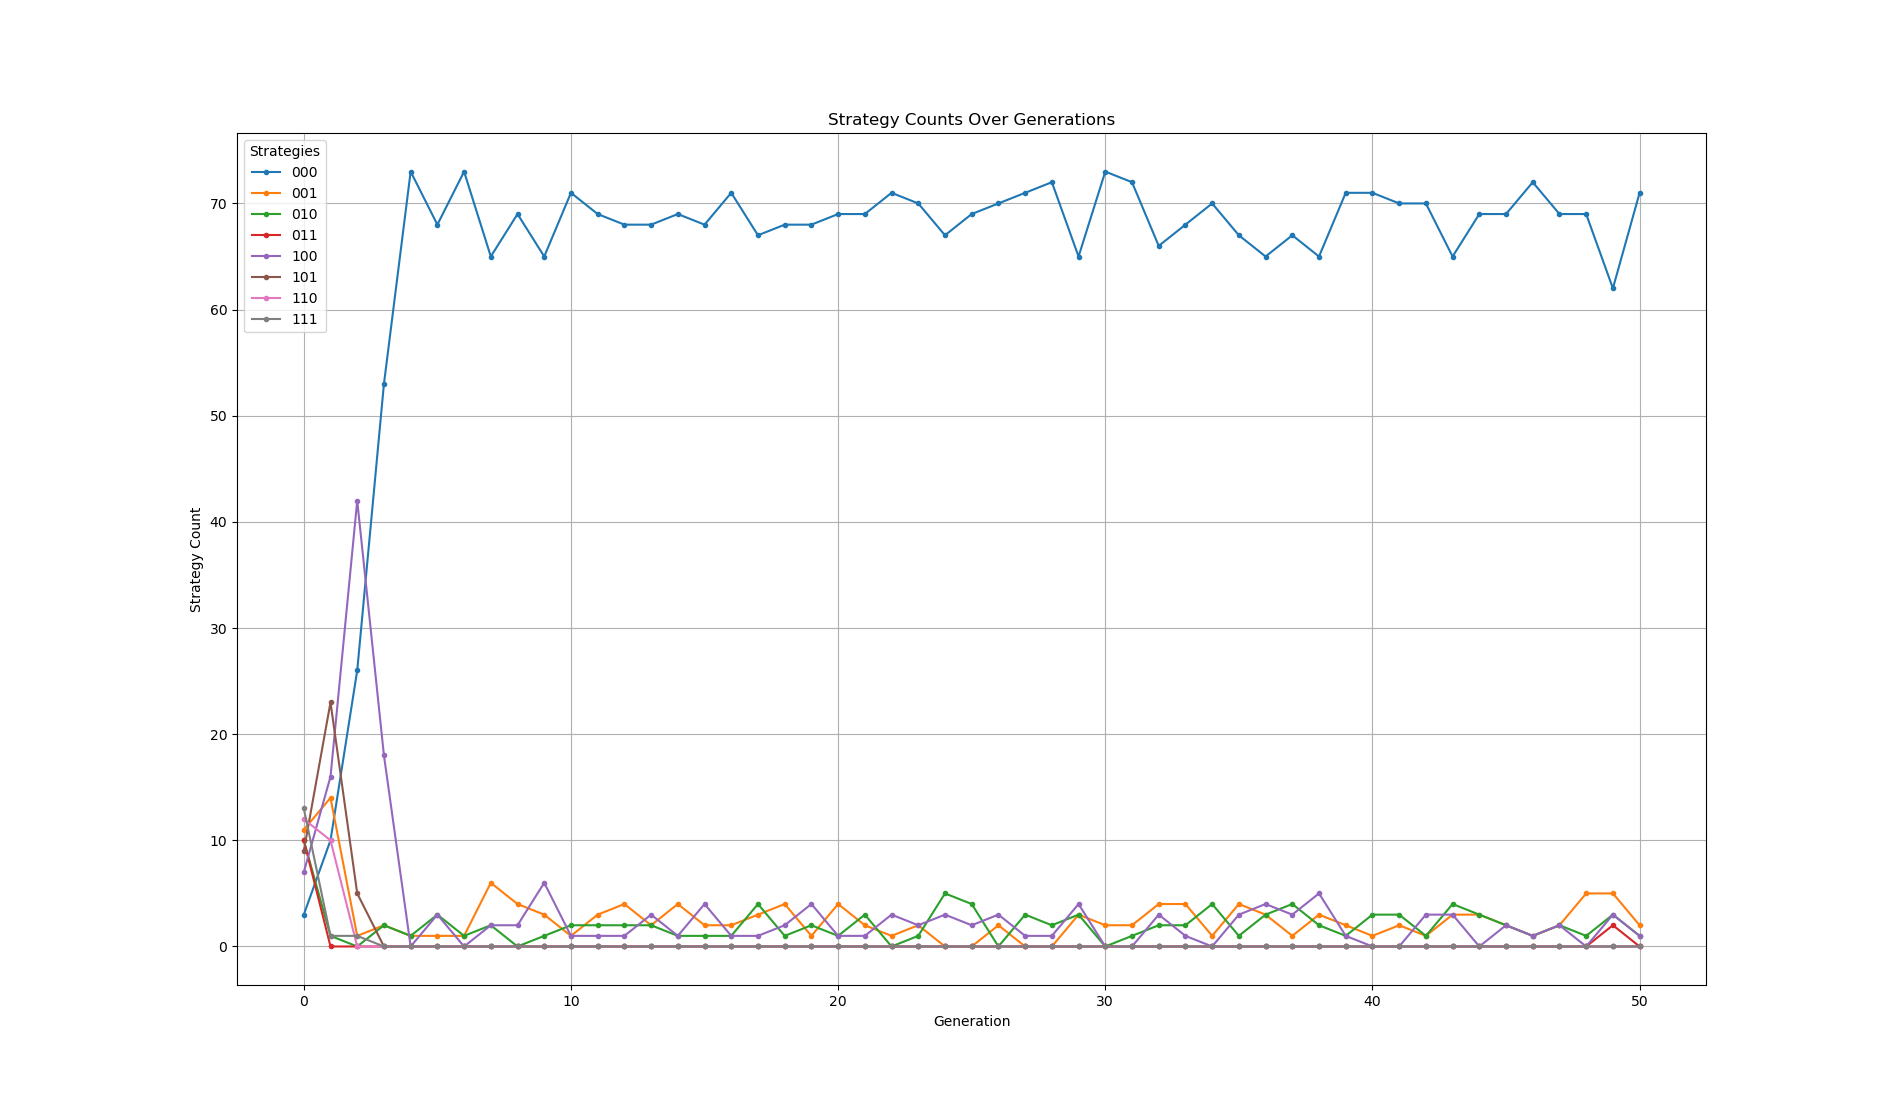
\includegraphics[width=\textwidth]{./images/defect_strats.png}
    \caption{Diversity of the strategy population over generations}
\end{figure}

\subsubsection{$1 \times $ Always Defect, $2 \times$ Always Co-Operate, \& $1 \times$ Tit-for-Tat}
\begin{code}
\begin{minted}[linenos, breaklines, frame=single]{text}
Best strategy: [0, 1, 0]
Fitness: 125
Generation: 0
[0, 0, 0]: 124
[0, 0, 1]: 99
[0, 1, 0]: 125
[0, 1, 1]: 94
[1, 0, 0]: 121
[1, 0, 1]: 99
[1, 1, 0]: 122
[1, 1, 1]: 90
\end{minted}
\caption{$1 \times $ always defect, $2 \times$ always co-operate, \& $1 \times$ tit-for-tat}
\end{code}

When a second Always Co-Operate is added to the mix, the best strategy reverts to being defect on the first move, then do the opposite of what the opponent did, for the same reasons as previously explored.

\begin{figure}[H]
    \centering
    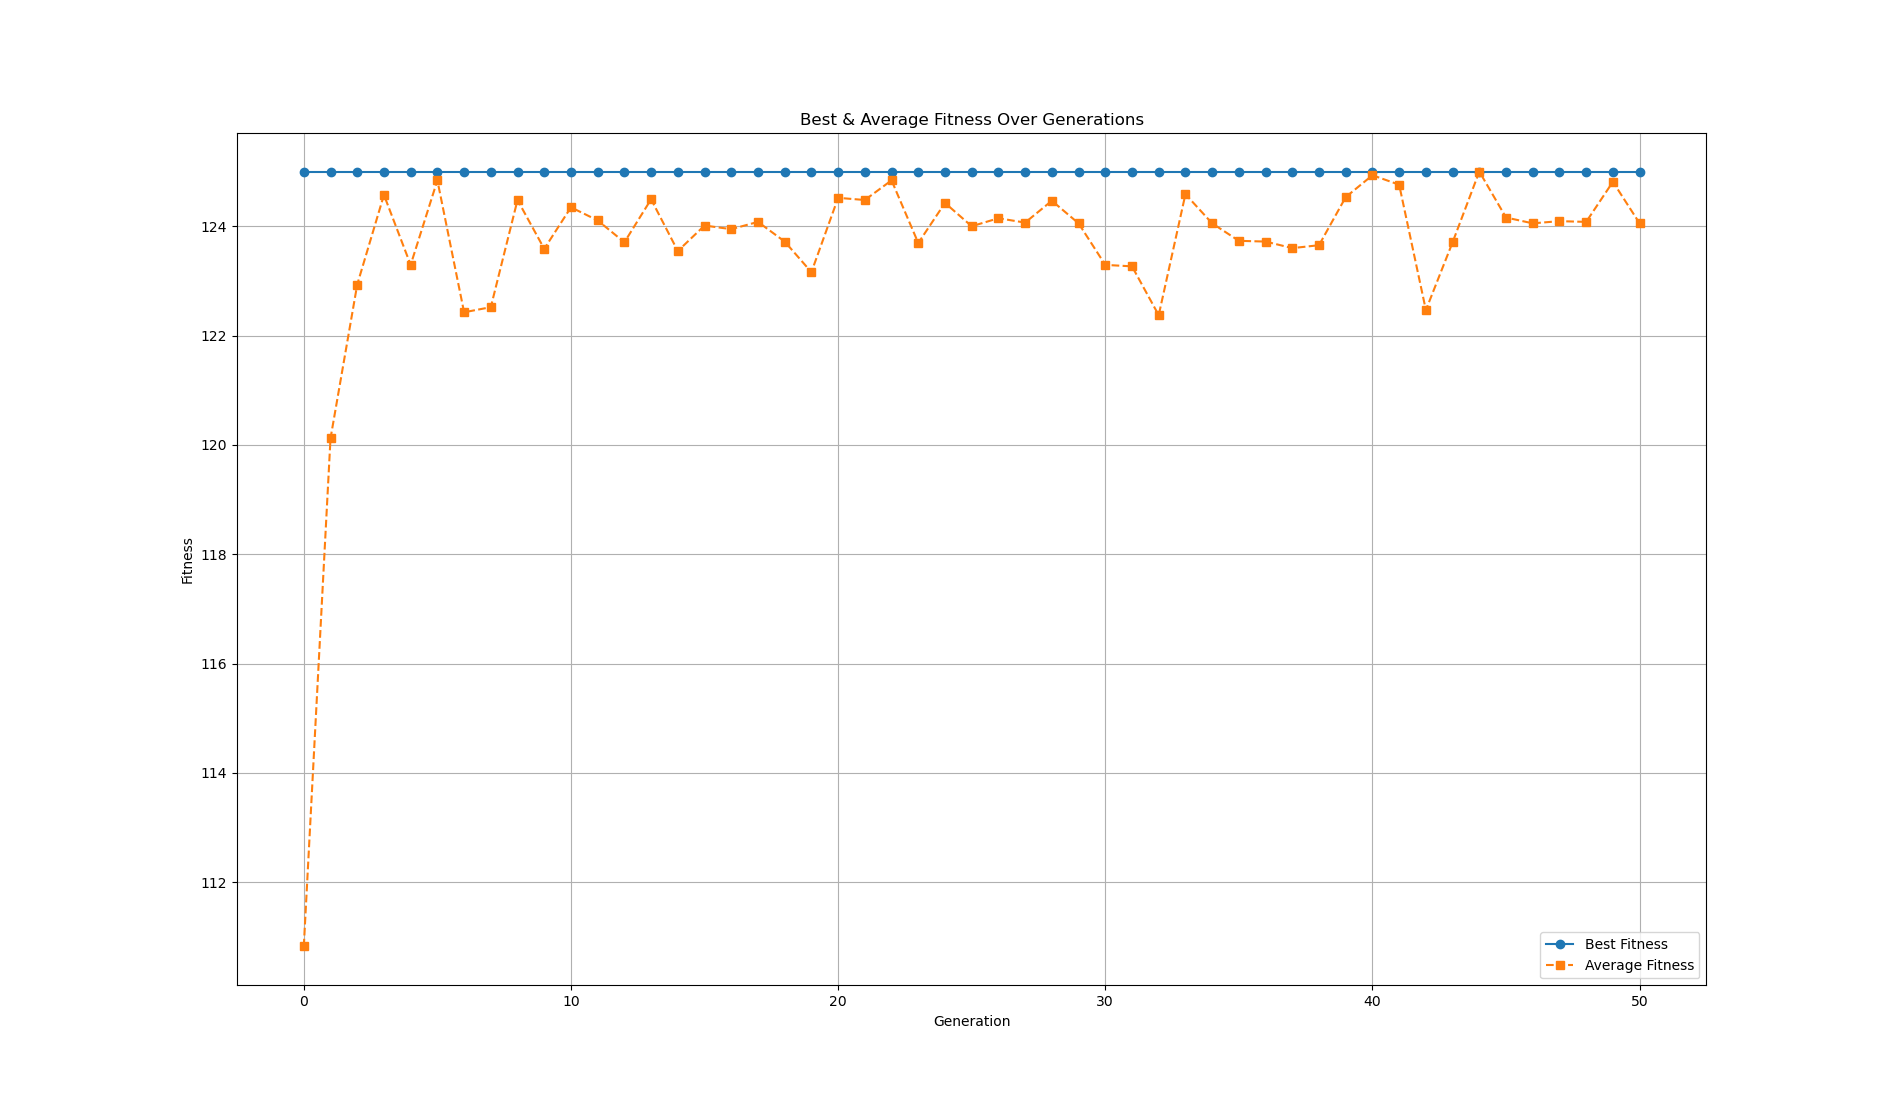
\includegraphics[width=\textwidth]{./images/cop_fitness.png}
    \caption{Fitness over generations}
\end{figure}

\begin{figure}[H]
    \centering
    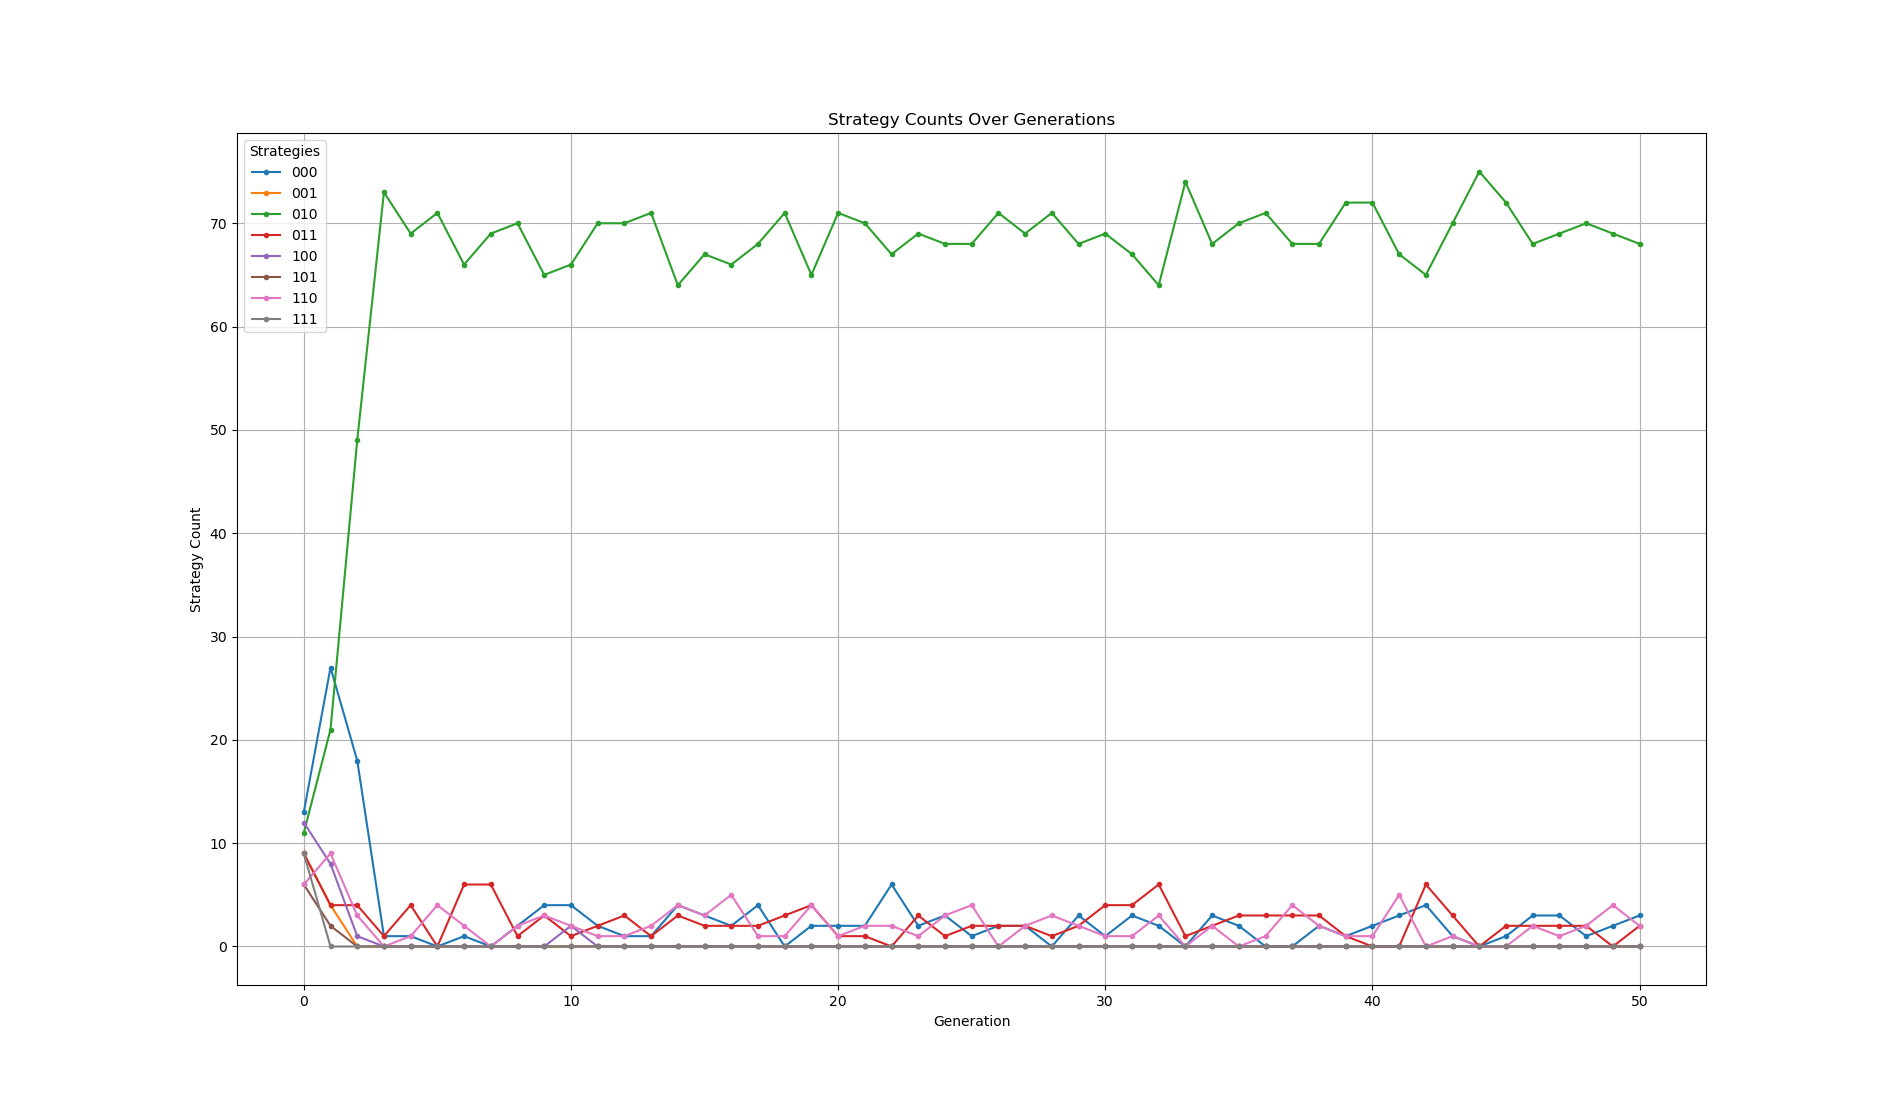
\includegraphics[width=\textwidth]{./images/cop_strats.png}
    \caption{Diversity of the strategy population over generations}
\end{figure}

\subsubsection{$1 \times $ Always Defect, $1 \times$ Always Co-Operate, \& $3 \times$ Tit-for-Tat}
\begin{code}
\begin{minted}[linenos, breaklines, frame=single]{text}
Best strategy: [1, 0, 1]
Fitness: 129
Generation: 0
[0, 0, 0]: 102
[0, 0, 1]: 117
[0, 1, 0]: 123
[0, 1, 1]: 120
[1, 0, 0]: 105
[1, 0, 1]: 129
[1, 1, 0]: 126
[1, 1, 1]: 120
\end{minted}
\caption{ $1 \times $ always defect, $1 \times$ always co-operate, \& $3 \times$ tit-for-tat} \end{code}
\end{code}

When three Tit-for-Tats are added into the mix, we see Tit-for-Tat emerge as the dominant strategy, which is to be expected;
it achieves a steady middle-ground approach via co-operation, and it has enough fellow co-operators to make up for the defection it suffers.
The defector strategies get punished frequently enough to reduce their winnings from defection, allowing co-operation to become a dominant \& winning strategy.

\begin{figure}[H]
    \centering
    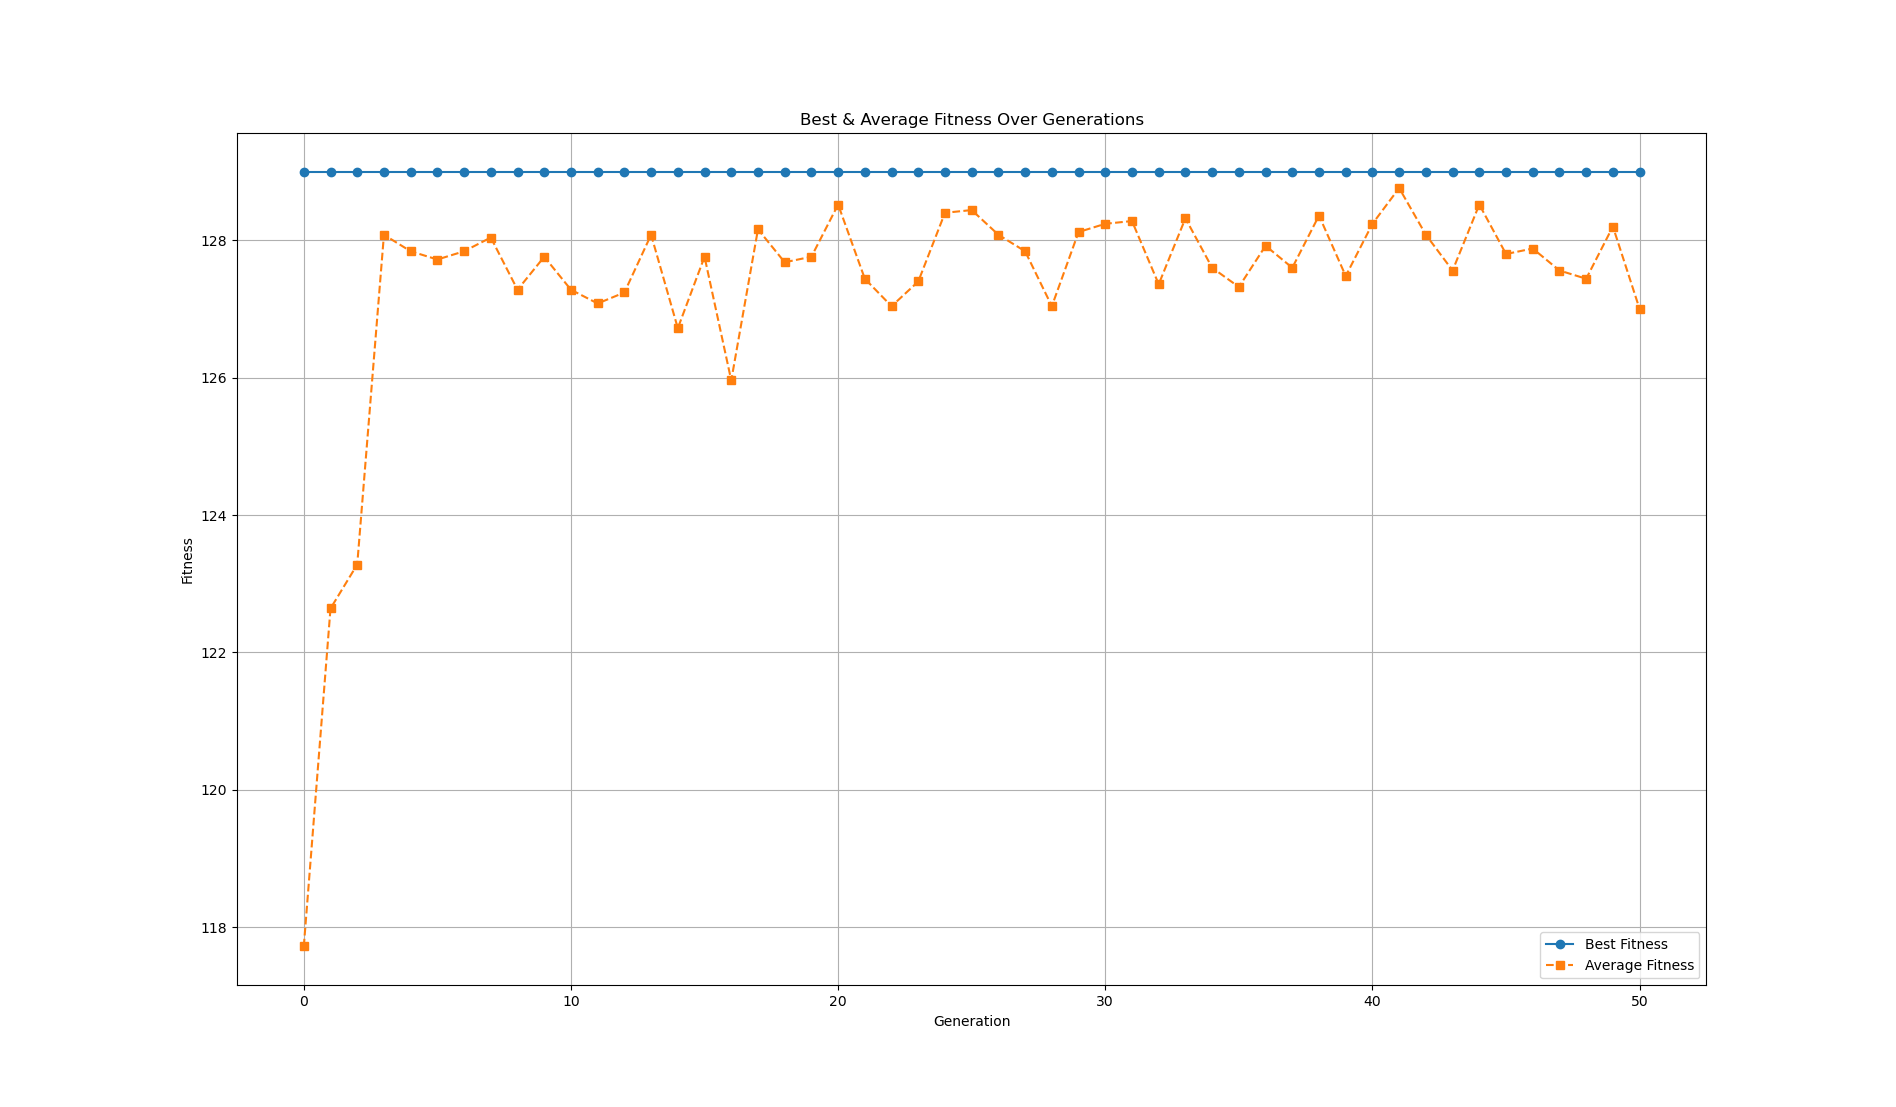
\includegraphics[width=\textwidth]{./images/tit_fitness.png}
    \caption{Fitness over generations}
\end{figure}

\begin{figure}[H]
    \centering
    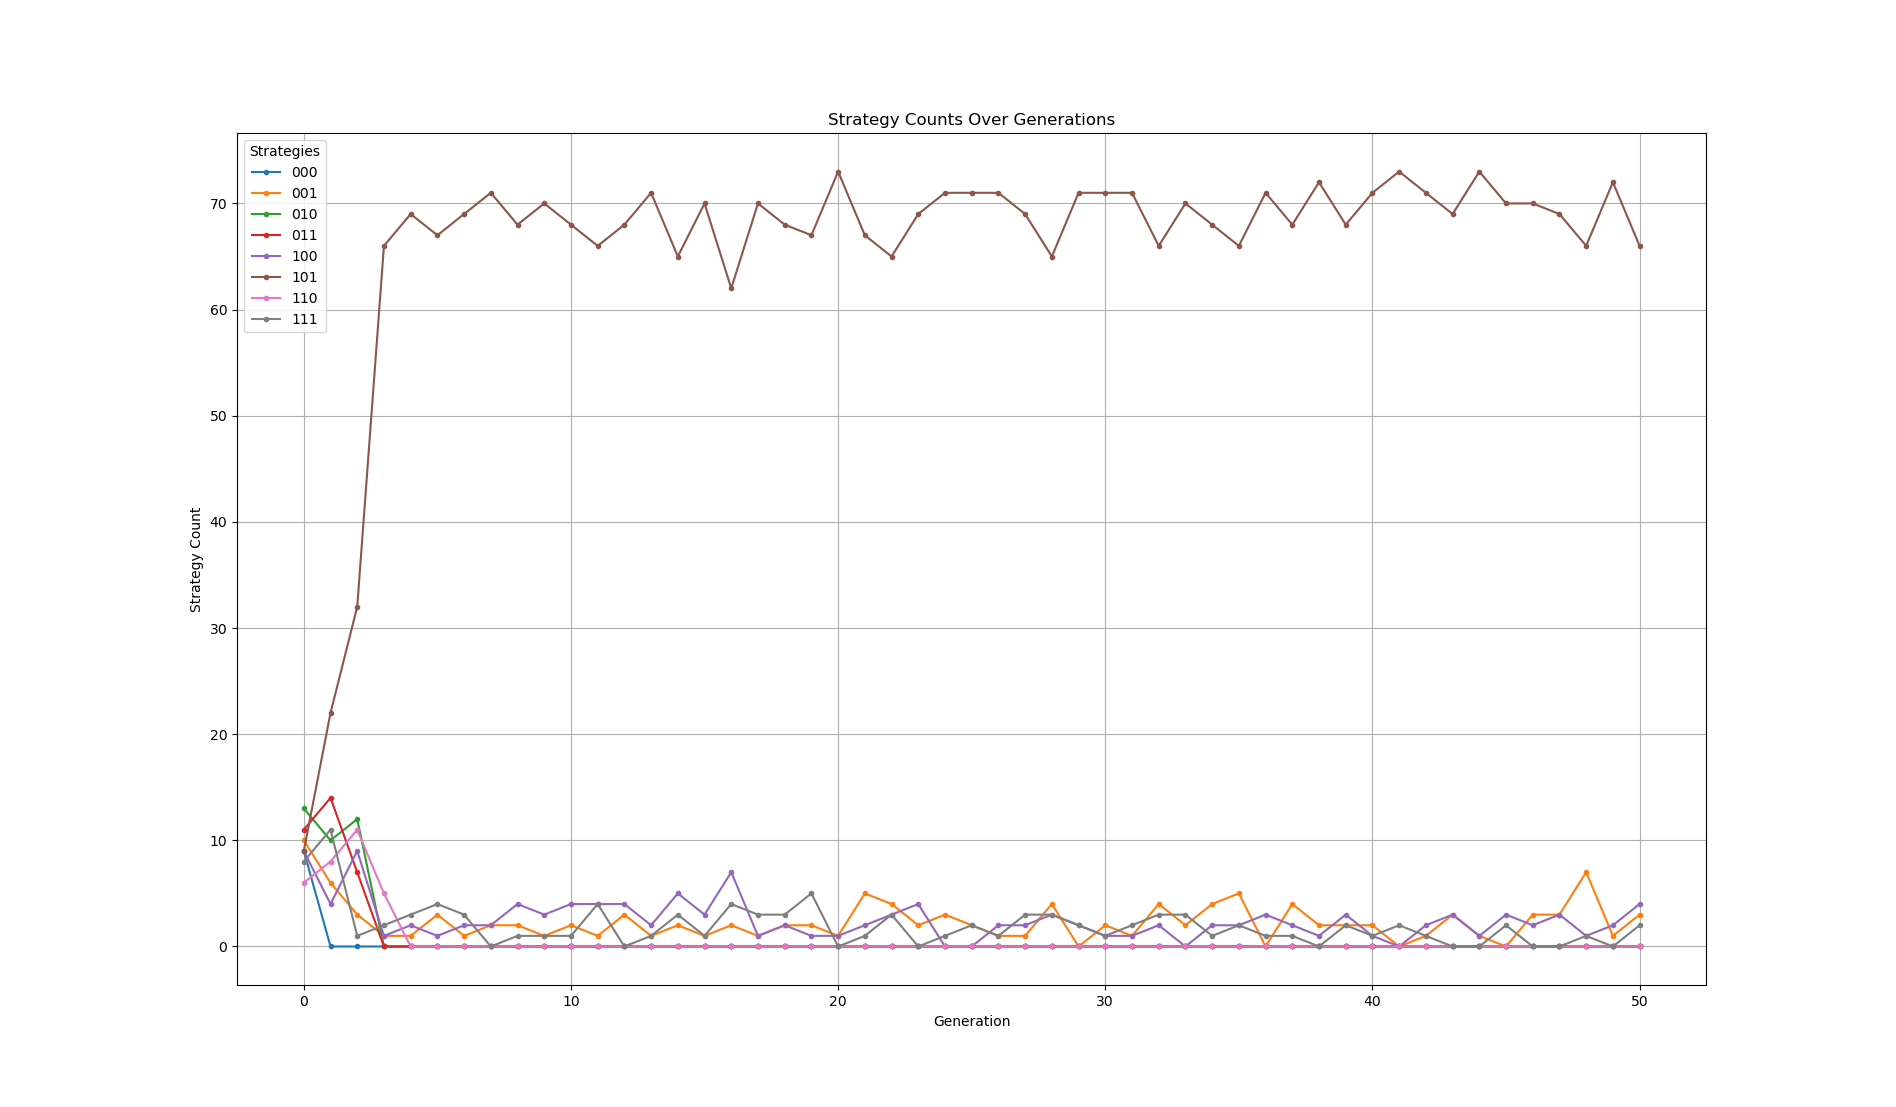
\includegraphics[width=\textwidth]{./images/tit_strats.png}
    \caption{Diversity of the strategy population over generations}
\end{figure}

\section{Part 2: Extension}
To extend the genetic algorithm implementation, I chose to add a variable level of noise to the program, supplied via command-line argument \mintinline{shell}{-n, --noise-level NOISE_LEVEL}. 
I then re-ran the same experiments as before with varying noise levels.

\subsection{\mintinline{shell}{NOISE_LEVEL = 0.1}}
The results that I got for each of the previously-attempted experiments when I set the noise level to 0.1 were as follows:
\begin{itemize}
    \item   \textbf{Equally proportioned:} \verb|[0,0,0]|.
    \item   \textbf{$2 \times$ always defect:} \verb|[0,0,0]|.
    \item   \textbf{$2 \times$ always co-operate:} \verb|[0,0,0]|.
    \item   \textbf{$3 \times$ tit-for-tat:} \verb|[1,0,1]|.
\end{itemize}

\subsection{\mintinline{shell}{NOISE_LEVEL = 0.2}}
The results that I got for each of the previously-attempted experiments when I set the noise level to 0.2 were as follows:
\begin{itemize}
    \item   \textbf{Equally proportioned:} \verb|[0,0,0]|.
    \item   \textbf{$2 \times$ always defect:} \verb|[0,0,0]|.
    \item   \textbf{$2 \times$ always co-operate:} \verb|[0,0,0]|.
    \item   \textbf{$3 \times$ tit-for-tat:} \verb|[0,0,0]|.
\end{itemize}

\subsection{\mintinline{shell}{NOISE_LEVEL = 0.5}}
The results that I got for each of the previously-attempted experiments when I set the noise level to 0.5 were as follows:
\begin{itemize}
    \item   \textbf{Equally proportioned:} \verb|[0,0,0]|.
    \item   \textbf{$2 \times$ always defect:}  \verb|[0,0,0]|.
    \item   \textbf{$2 \times$ always co-operate:} \verb|[0,0,0]|.
    \item   \textbf{$3 \times$ tit-for-tat:} \verb|[0,0,0]|.
\end{itemize}
\subsection{\mintinline{shell}{NOISE_LEVEL = 0.8}}
The results that I got for each of the previously-attempted experiments when I set the noise level to 0.8 were as follows:
\begin{itemize}
    \item   \textbf{Equally proportioned:} \verb|[0, 0, 0]|.
    \item   \textbf{$2 \times$ always defect:} \verb|[0,0,0]|.
    \item   \textbf{$2 \times$ always co-operate:} \verb|[0,0,0]|.
    \item   \textbf{$3 \times$ tit-for-tat:} \verb|[0,0,0]|.
\end{itemize}

As can be seen from the above outputs, the introduction of even just a little noise to each evolution immediately broke any possibility for co-operation, the one exception being that tit-for-tat still performed well against three other tit-for-tats at the lowest noise level, most likely because it got some co-operation in before noise disrupted the chain of co-operation.
Noise makes co-operation more difficult, and is highly detrimental to these simple strategies defined by short bitstrings: 
these genomes don't have the necessary complexity to express a level of forgiveness, so one one bit of noise can destroy all chances of co-operation for the rest of the game.
For a noisy environment, error-tolerant strategies are required, like generous tit-for-tat, which can avoid falling into the defection loops that overly rigid and/or grudging strategies fall into.

\end{document}
